\section{Operational Carbon Footprint Analysis}
Operation Carbon Footprint is the most important metric for the goal of our observation, since it is the result of combining energy usage (related to power consumption) and carbon intensity. \\
For this reason we will see a combination of the observations we did related both to power and CI.

\vspace{-15pt}

\begin{figure}[H]
\centering
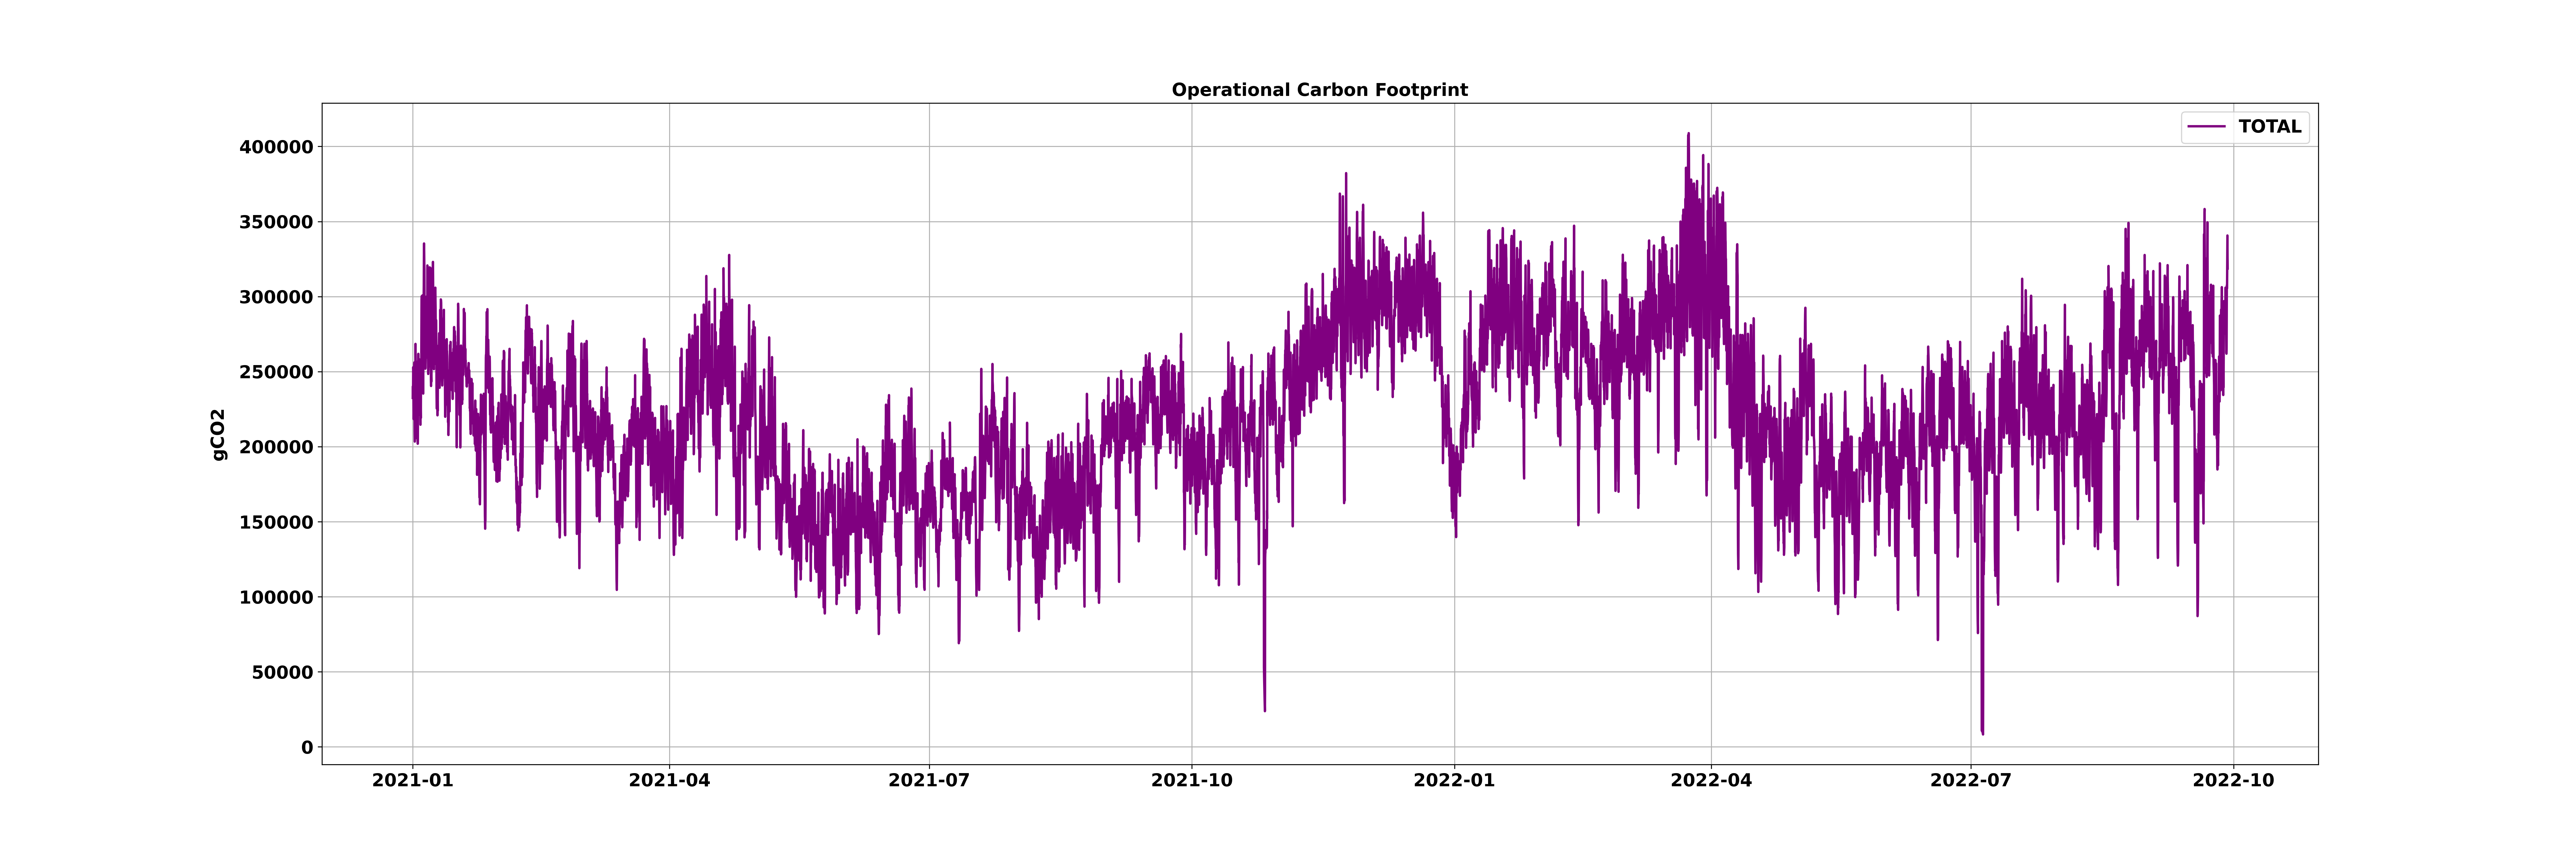
\includegraphics[width=1\textwidth]{../../PLOTS/Cop_total.png}
\captionsetup{skip=-10pt}
\caption{Cop total value (sum of all nodes in the server)}
\label{fig:Cop_total}
\end{figure}

\begin{center}
\setstretch{0.9}
count     15263.000000 \\
mean     220186.340067 \\
std       54400.325364 \\
min        8292.258962 \\
25\%      181522.725893 \\
50\%      218140.616056 \\
75\%      258846.427357 \\
max      408868.699240   
\end{center}

\subsection{Cop r206n01 STL}

\vspace{-10pt}

\begin{figure}[H]
\centering
\includegraphics[width=1\textwidth]{../../PLOTS/Cop_stl.png}
\caption{Cop r206n01 STL}
\label{fig:Cop_r206n01_stl}
\end{figure}

\subsection{Cop analysis using Meta's Prophet}


\vspace{-10pt}

\begin{figure}[H]
\centering
\includegraphics[width=1\textwidth]{../../PLOTS/Cop_prophet.png}
\caption{Cop trends}
\label{fig:Cop_prophet}
\end{figure}